\documentclass[a4paper,12pt]{scrartcl}

\usepackage{exercice_sheet}

%\trait
%\section*{}
%\exo{}
%\question{}
%\subquestion{}

\date{}


% Title Page
\title{Loi binomiale, corrigé des exercices}

\author{\textsc{Mathématiques}}

\begin{document}

\maketitle

%\tableofcontents

\exo{Loi binomiale $\mathcal{B}(10;0.2)$}

\question{}
En utilisant la formule donnée au début du cours $P(X=k) = C_n^k p^k (1-p)^{n-k}$:

$P(X=3) = C_{10}^3 \times 0.2^3 \times 0.8^7 = 0.2013$.

\question{}
$P(X \leqslant 3) = 0.8791$

\question{}
Les événements $X \leqslant 3$ et $X>3$ sont complémentaires, c'est-à-dire que la somme de leurs probabilités est 1. On a donc $P(X>3) = 1 - P(X \leqslant 3) = 0.1209$.

\question{}
$E(X) = np = 2$ et $\sigma(X) = \sqrt{np(1-p)} = 1.2649$.

\exo{Loi binomiale $\mathcal{B}(15;0.4)$}

\question{}
$P(X = 5) = 0.1859$

\question{}
$P(X \leqslant 14) = 0.0000$. En réalité, le résultat n'est pas rigoureusement nul, mais sa valeur est tellement proche de 0 que son arrondi à $10^{-4}$ est 0.

\question{}
$P(X < 14) = 1.0000$. de la même façon qu'à la question précédente, le résultat n'est pas exactement égal à 1, mais le résultat arrondi est celui-ci.

\question{}
$E(X) = np = 6$ et $\sigma(X) = \sqrt{np(1-p)} = 1.8974$.

\exo{Machines en panne}

\question{}

Pour justifier que $X$ suit une loi binomiale, il suffit de reprendre les 3 points indiquée dans le cours.

\begin{itemize}
    \item X mesure le nombre de machines en panne. Il y a donc deux issues possibles (en panne ou pas en panne);
    \item Toutes les machines sont identiques et le fait qu'une tombe en panne n'influe pas sur la fiabilité des autres;
    \item On considère 100 machines.
\end{itemize}

Le nombre de machines en panne sur 100, $X$, suit donc une loi binomiale $\mathcal{B}(100;0.03)$.

\question{}
$P(X=6) = 0.0496$.

\question{}
$P(X \leqslant 2) = 0.4198$.

\question{}
Cela revient à dire que 0, 1 ou 2 machines sont tombées en panne ce mois-ci. Cela revient donc à calculer $P(X \leqslant 2)$.

$P(X \leqslant 2) = 0.4198$ (question précédente).

\exo{}

\question{}

\begin{itemize}
    \item $X$ mesure le nombre de personnes ayant suivi la formation. Il y a donc deux issues possibles (a suivi ou n'a pas suivi);
    \item On considère l'effectif assez grand pour considérer qu'il s'agit d'un tirage avec remise;
    \item On tire au hasard 15 personnes.
\end{itemize}

$X$ suit donc une loi binomiale de paramètre 15 et 0.3: $\mathcal{B}(15;0.3)$.

\question{}
Il s'agit de déterminer la probabilité $P(X=3)$.

$P(X=3) = C_{15}^3 \times 0.3^3 \times 0.7^{12} = 0.17$.

\question{}
\og{}Une personne au plus \fg{} signifie \og{}Au maximum une personne \fg{}. Cela revient donc à calculer $P(X \leqslant 1) = 0.04$.

\exo{trouver $n$}
Ici, l'exercice est inversé. On ne connaît qu'un sur deux des paramètres de la loi (on connaît $p$ mais $n$ est inconnu) mais on connaît la probabilité limite que l'on souhaite (0.008). Si on reprend la formule de la loi binomiale, l'inéquation de l'énoncé est équivalente à:

\begin{equation*}
 C_n^0 \times 0.2^0 \times 0.8^n \leqslant 0.008
\end{equation*}

Or, $C_n^0 = 1, \forall n \in \mathbb{N}$ et $0.2^0 = 1$. L'équation se simplifie donc en:

\begin{equation*}
 0.8^n \leqslant 0.008
\end{equation*}

$\Leftrightarrow \ln(0.8^n) \leqslant \ln(0.008)$

$\Leftrightarrow n \geqslant \dfrac{\ln(0.008)}{\ln(0.8)}$ (l'inégalité change de sens car $\ln 0.8 < 0$)

$\Leftrightarrow n \geqslant 21.6$

$\Leftrightarrow n \geqslant 22$ (car $n \in \mathbb{N}$)

Donc à partir de $n = 22$, $P(X=0) \leqslant 0.008$. 

\exo{Le cancre}

\question{}

\subquestion{}
Il y a 3 réponses proposées pour une réponse juste. Donc $p = \frac{1}{3}$.

\subquestion{}
Il y a 5 questions, avec une probabilité de succès de $\frac{1}{3}$. $X$ suit donc une loi binomiale de paramètres $\mathcal{B} \left(5;\frac{1}{3} \right)$.

\subquestion{}
Cela revient à calculer $P(X=5) = C_5^5 \times \left(\frac{1}{3}\right)^5 \times \left(\frac{2}{3}\right)^0 = \frac{1}{3^5} = \frac{1}{243} \approx 0.0041$.

\subquestion{Loi de probabilité}

On calcule $P(X=0), P(X=1), \ldots P(X=5)$ et on compile le résultat comme dans la table \ref{tab:truc}.

\begin{table}[h]
\centering
\begin{tabular}{|l|l|l|l|l|l|l|}
\hline
$x_i$        & 0     & 1     & 2     & 3     & 4     & 5     \\ \hline
$P(X = x_i)$ & 0.132 & 0.329 & 0.329 & 0.165 & 0.041 & 0.004 \\ \hline
\end{tabular}
\caption{Tableau des probabilités de la loi binomiale $\mathcal{B}\left(5;\frac{1}{3}\right)$.}
\label{tab:truc}
\end{table}

\subquestion{Espérance et écart-type}
$E(X) = np = \frac{5}{3} \approx 1.67$ et $\sigma(X) = \sqrt{np(1-p)} = \sqrt{5 \times \frac{1}{3} \times \frac{2}{3}} \approx 1.05$. 

\question{La variable $Y$.}

\subquestion{}
Si $X$ est le nombre de réponses justes, alors $5-X$ est le nombre de réponses fausses. Ainsi, sachant qu'une réponse juste rapporte 1 point et qu'une réponse fausse retire 0.5 points, $Y = X - 0.5 \times (5-X) = 1.5X-2.5$.

Les valeurs possibles pour $Y$ sont donc:

\begin{tabular}{|l|l|l|l|l|l|l|}
\hline
$X$        & 0     & 1     & 2     & 3     & 4     & 5     \\ \hline
$Y$        &-2.5   &-1     & 0.5   & 2     & 3.5   & 5
 \\ \hline
\end{tabular}

\subquestion{}
On obtient donc le tableau de probabilités suivant:

\begin{table}[h]
\centering
\begin{tabular}{|l|l|l|l|l|l|l|}
\hline
$y_i$        &-2.5   &-1     & 0.5   & 2     & 3.5   & 5     \\ \hline
$P(Y=y_i)$  & 0.132 & 0.329 & 0.329 & 0.165 & 0.041 & 0.004
 \\ \hline
\end{tabular}
 \caption{Variable $Y$.}
 \label{tab:y}
\end{table}

\subquestion{}
La probabilité d'obtenir une note positive s'écrit $P(Y \geqslant 0)$. Il suffit d'additionner les probabilités correspondantes du tableau \ref{tab:y}.

$P(Y \geqslant 0) = 0.539$.

\subquestion{}
Attention, $X$ suit une loi binomiale, mais ce n'est \emph{pas} le cas de $Y$. 

Par contre, $Y$ est une transformation affine de la variable $X$. On peut donc déduire son espérance et son écart-type de ceux de $X$.

On a donc $E(Y) = 1.5 \times E(X) - 2.5 = 0$ et $\sigma(Y) = 1.5 \times \sigma(X) = 1.58$.

\question{La variable $Z$.}

\subquestion{}
Les valeurs possibles pour $Z$ sont 0, 0.5, 2, 3.5 et 5.

\subquestion{}
\begin{tabular}{|l|l|l|l|l|l|l|}
\hline
$z_i$       & 0     & 0.5   & 2     & 3.5   & 5     \\ \hline
$P(Z=z_i)$  & 0.461 & 0.329 & 0.165 & 0.041 & 0.0041
 \\ \hline
\end{tabular}

\subquestion{}
Espérance:
\begin{equation*}
 E(Z) = 0 \times 0.461 + \ldots + 5 \times 0.0041 \approx 0.658
\end{equation*}

Écart-type: on commencera par calculer la variance $V(Z) = E(Z^2) - E^2(Z)$. On obtient $V(Z) = 0.914$ d'où $\sigma(Z) = \sqrt{V(Z)} = 0.956$.

\exo{Mazout}

Dans cet exercice pour appliquer la loi binomiale, on doit considérer que la population totale de 20000 piafs est assez importante pour que l'expérience s'apparente à un tirage sans remise. 

500 sternes parmi 20000 furent baguées. La probabilité d'en prélever une baguée est donc de $\frac{500}{20000} = \frac{1}{40}$. 

Le nombre de sternes baguées (appelons $X$ la variable comptant le nombre d'oiseaux bagués) sur un prélèvement de 100 suit donc la loi $\mathcal{B}\left( 100 ; \frac{1}{40}\right)$.

\question{}
Cela revient à calculer $P(X=0)$. On obtient $P(X=0) = 0.0795$

\question{}
Cela revient à calculer $P(X \geqslant 2)$. On obtient $P(X \geqslant 2) = 0.7166$

\exo{Accidents}

\question{}
Le nombre de jeunes conducteurs ayant eu un accident durant l'année parmi 10 ($X$) suit la loi binomiale $\mathcal{B}\left(10 ; 0.4\right)$

\begin{equation*}
 P(X \geqslant 1) = 0.994
\end{equation*}


\question{}
Le nombre de conducteurs pas jeunes ayant eu un accident durant l'année parmi 10 ($X$) suit la loi binomiale $\mathcal{B}\left(10 ; 0.125\right)$

\begin{equation*}
 P(X \geqslant 1) = 0.737
\end{equation*}

\question{}

\subquestion{}
À noter qu'ici, il n'est plus question de loi binomiale mais de probabilités générales.

On peut modéliser la situation à l'aide d'un un arbre de probabilités (figure \ref{fig:tree}):

\begin{figure}[h]
\begin{center}
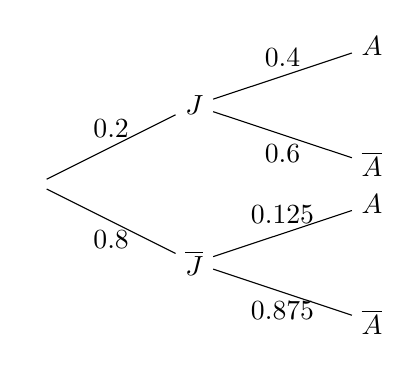
\begin{tikzpicture}
     \tikzstyle{level 1}=[level distance=2cm, sibling distance=2cm]
     \tikzstyle{level 2}=[level distance=2cm, sibling distance=1.5cm]
     \node{}[grow=right]
     child{node{$\overline{J}$}
     child{node[right]{$\overline{A}$}
edge from parent node[below]{$0.875$}}
     child{node[right]{$A$}
edge from parent node[above]{$0.125$}}
     edge from parent node[below]{$0.8$}}
     child{node{$J$}
     child{node[right]{$\overline{A}$}
edge from parent node[below]{$0.6$}}
     child{node[right]{$A$}
edge from parent node[above]{$0.4$}}
     edge from parent node[above]{$0.2$}};
\end{tikzpicture} 
\end{center}
\caption{Arbre de probabilité modélisant la situation proposée.}
\label{fig:tree}
\end{figure}

On voit ainsi que $p = P(A) = 0.2 \times 0.4 + 0.8 \times 0.125 = 0.18$.

\subquestion{}
Si on appelle $X$ la variable comptant le nombre d'assurés ayant eu au moins un accident, $X$ suit une loi normale $\mathcal{B}\left( 10 ; 0.18 \right)$. 

On a donc $P(X \geqslant 1) = 0.8626$.

\end{document}



